\documentclass[a4paper,11pt]{report}
\usepackage{coverstory,times,epsfig,calc}
\usepackage{amsmath,amssymb}
\usepackage{cite}
\usepackage{caption}
\usepackage{floatrow}   
\usepackage{subcaption}
\usepackage{graphicx,xcolor} 
\usepackage{lscape}
%\usepackage{hyperref}
\usepackage{epsfig} % for postscript graphics files
\usepackage{graphicx}
\usepackage{multirow}
\usepackage{tabu}
\usepackage{floatrow}
\usepackage{url}
\usepackage{easybmat}
\usepackage{kotex}
\usepackage{IEEEtrantools}
\usepackage[a4paper,left=35mm,right=35mm,top=53mm,bottom=53mm]{geometry}

\floatsetup[table]{capposition=top}
\setcounter{secnumdepth}{3}
%\usepackage{hhline}
%\usepackage{multirow}
%\usepackage{rotating}
%\usepackage{booktabs}
%\usepackage[hang,flushmargin]{footmisc}
%\usepackage{float}
%\usepackage{amsbsy}
%\usepackage{url}
%\usepackage{pifont}
%\usepackage{mathptmx} % assumes new font selection scheme installed
%\usepackage{longtable}
%\usepackage{grad,times,graphicx,calc}

%\usepackage{fancyhdr}
%\usepackage{graphics} % for pdf, bitmapped graphics files
%%%%%%%%%%%%%%%%%%%%%%%%%%%%%%%%%%%%%%%%%%%%%%%%%%%%%%%%%%%%%%%%%%%%%%%%%%%%%%%%%%%%APPENDIX EDIT
\newenvironment{myEnumerate}{
\begin{enumerate}
  \setlength{\itemsep}{0pt}
  \setlength{\parskip}{0pt}
  \setlength{\parsep}{0pt}}
{\end{enumerate}
}
%\Urlmuskip=0mu plus 1mu
\newif\ifappendixin
\makeatletter
  \renewcommand{\appendix}{\par
    \@ifundefined{appendixin}{\appendixintrue}{\appendixinfalse}
    \setcounter{chapter}{0}%
    \setcounter{section}{0}%
    \setcounter{subsection}{0}%
    \setcounter{figure}{0}%
    \def\@chapapp{\appendixname}%
    \def\thechapter{\Alph{chapter}}%
    %\def\thesection{\Alph{chapter}.(\roman{section})}%
    \def\thesection{\Alph{chapter}.\arabic{section}}%
    \renewcommand\section{%
                \@startsection {section}{1}{\z@}%
                {-3.5ex \@plus -1ex \@minus -.2ex}%
                {2.3ex \@plus.2ex}%
                {\normalfont\Large\bfseries}}
    \renewcommand\thefigure{%
                \ifnum \c@section>\z@ \Alph{chapter}.\fi \@arabic\c@figure}
    \renewcommand\theequation{%
                \ifnum \c@section>\z@ \Alph{chapter}.\fi \@arabic\c@equation}
    \renewcommand\thetable{%
                \ifnum \c@section>\z@ \Alph{chapter}.\fi \@arabic\c@table}
}

\makeatother


%%%%%%%%%%%%%%%%%%%%%%%%%%%%%%%%%%%%%%%%%%%%%%%%%%%%%%%%%%%%%%%%%%%%%%%%%%%%%%%%%%%%APPENDIX EDIT
\renewcommand{\baselinestretch}{1}
\renewcommand{\arraystretch}{1.3}

\newtheorem{theorem}{Theorem}
\newtheorem{example}{Example}
\newtheorem{lemma}{Lemma}
\newtheorem{corollary}{Corollary}
\newtheorem{definition}{Definition}
\newtheorem{conjecture}{Conjecture}
\newcommand{\rmnum}[1]{\romannumeral #1}
\newcommand\MyLBrace[2]{\left.\rule{0pt}{#1}\right\}\text{#2}}
\newcommand\bovermat[2]{%
	\makebox[0pt][l]{$\smash{\overbrace{\phantom{%
					\begin{matrix}#2\end{matrix}}}^{\text{#1}}}$}#2}

%%%%%%%%%%%%%%%%%%%%%%%%%%%%%%%%%%%%%%%%%%%%%%%%%%%%%%%%%%%%%%%%%%%%%%%%%%%%%%%%%%%%
\title{Improving the Triplet Network for Wi-Fi Based Handwritten Signature Verification}

\author{Young-Woong Kwon}
\date{December 2019}

\begin{document}
\makecover
\maketitle

\signaturepage

\pagestyle{plain}
\baselineskip 8.5mm
\newpage
{\LARGE \bf
\noindent ACKNOWLEDGEMENT}\\[11pt]
\vskip 1em \pagestyle{empty}
\renewcommand{\baselinestretch}{0.85}

\begin{flushright}
{October 2019 \\ \textbf{Young-Woong Kwon}}
\renewcommand{\baselinestretch}{1.0}
\end{flushright}
 \pagestyle{plain}
%\acknowledgement
%\input{thanks2}
%%%%%%%%%%%%%%%%%%%%%%%%%%%%%%%%%%%%%%%%%%%%%%%%%%%%%%%%%%%%%%%%%%%%%% �������
\pagenumbering{roman} % Page Numbering style
\setcounter{page}{0}
\tableofcontents
\listoffigures
\addcontentsline{toc}{chapter}{\protect\numberline{}
    \hspace*{-0.29in} List of Figures}
\listoftables
\addcontentsline{toc}{chapter}{\protect\numberline{}
    \hspace*{-0.29in} List of Tables}

\begin{abstract}
\addcontentsline{toc}{chapter}{\protect\numberline{}
    \hspace*{-0.29in} Abstract}
\begin{center}
	\LARGE Improving the Triplet Network for Wi-Fi Based Handwritten Signature Verification
\end{center}

\parbox[t]{0.4\textwidth}

{
	\begin{flushright}
		Young-Woong Kwon\\
		School of Electrical and Electronic Engineering\\
		The Graduate School\\
		Yonsei University
	\end{flushright}
}
\vspace{0.1em}

Identity verification using Wi-Fi signals is a challenging task since the shape of the signal varies according both the orientation and the position of the user. In this thesis, a system for identity verification is developed based on the hand gesture signature signals sensed by the Wi-Fi Channel State Information (``CSI'').
A three-channel ConvNet structure is adopted to learn the discriminative features based on a relatively small size in-air handwritten signature dataset. We propose an input triplet mining based on the kernel and range space learning to improve the convergence speed of the triplet network training.
Our experimental results on the Wi-Fi CSI signature dataset shows encouraging accuracy and convergence performances.

\vspace{\stretch{1}}
\noindent
\hrulefill\\
{\bf Key words : In-air handwritten signature verification, Wi-Fi Channel State Information, Triplet network, and the Kernel and Range space learning}
\parbox[t]{0.8\textwidth}
{}

\end{abstract}

\newpage
\pagenumbering{arabic} % Page Numbering style
\setcounter{page}{1}

\chapter{Introduction}\label{chapter:Introduction}
\section{Background}
% signature
Signatures written on paper have long been used as an identification tool, and various methods for verifying individuals have been developed~\cite{fahmy2010online,galbally2015line,sanmorino2012survey,sesa2012information}.
% biometric
As mobile devices increase, identity verification using biometrics traits is becoming more widely used.
Compared to the use of complex passwords, using biometric systems to user verification has advantages of increased security, convenience, and accountability~\cite{hutton2004biometrics}.
% camera sensor
With the development of various sensors such as depth camera and mobile camera, in-air signature has also become available~\cite{bailador2011analysis}. However, they had to use a special sensor prepared for signature. ~\cite{jeon2012system,malik20183dairsig} used depth camera, \cite{ketabdar2012magnetic} used mobile device to record position of hand.
% WiFI CSI
On the other hand, some studies use Wi-Fi CSI signals to identify the biometric characteristics of the human body. Since they use commercial devices that are already widespread, they do not need any special input devices.
~\cite{hong2016wfid,liu2015tracking,yousefi2017survey} studied CSI signals to identify the various biometrics characteristics of the body. ~\cite{abdelnasser2015wigest,nandakumar2014wi} used CSI signals to enable users to recognize their gestures.
% CSI signature
Recently, a study was conducted to identify signatures written in the air using CSI signals~\cite{moon2017air}. However, in this study, only the signals entered in one direction were recognized. Due to the nature of the in-air signature, which is difficult to specify the direction in which the signal is input, a verification system is required regardless of the direction in which the signal is entered.
% Deep learning
More recently, there have been studies using deep learning technology to characterize CSI signals. Deep Learning-based models are spotlighted for their automated feature extractors and superior classification capabilities based on them, compared to traditional handcraft models. Deep learning was used to recognize users based on the body shape~\cite{pokkunuru2018neuralwave}, or to identify them with the characteristics shown in their behavior~\cite{shi2017smart}.
% our methods
We used deep learning technology to create a system that can be identity-recognizable even for multi-way air signatures entered with Wi-Fi CSI.
The deep learning model used a triplet network to increase the accuracy of feature extraction while allowing accurate classification, and also improved the model's convergence speed using the kernel and range space running~\cite{toh2018gradient}.

%\newpage
\newpage
\section{Motivation and Contributions}
The main contributions of our work can be summarized as follows:
\begin{itemize}
\item Proposal of a system for identity verification based on the Wi-Fi handwritten signature signals using a deep triplet network.
\item Adopted the kernel and the range (KAR) space learning to mine the distinctive triplet inputs which boost the convergence speed of the training loss in the triplet network.
\item Provision of an experimental study using an in-house Wi-Fi handwritten signature dataset collected from 50 subjects.
\end{itemize}

\section{Organization of Thesis}
The paper is organized as follows: related works including the triplet network and KAR space learning are introduced in Section 2 for immediate reference. Our proposed method is discussed in Section 3. Section 4 describes our experimental results and analysis. Some concluding remarks are given in Section 5.
%

%\chapter{Preliminaries}\label{chapter:Preliminaries}
%\label{chp:Survey}

\section{ConvNets}
% description of convnet
Convolutional Neural Networks is a specal case of Multi Layer Perceptron and it has unified feature extractor and classifier in one network. It has been widely applied to visual objects such as image, video or 2D array input. Several factors make ConvNets attractive in image related tasks.
Local connectivity captures local correlation property of image. It is applycable by using ConvNet filter.Weight sharing helps to reduce the number of weights in feature maps.
Also, CUDA libraries makes the tranining feature maps easier to reduce training time.

%3.3. CSI
\section{Wi-FI Channel State Information}
CSI captures signal strength and phase information for OFDM subcarriers and between each pair of transmit-receive antennas.
It runs on a commodity 802.11n NIC and records Channel State Information (CSI based on the 802.11 standard.
The CSI contains information about the channel between sender and receiver at the level of individual data subcarriers, for each pair of transmit and receive antennas.
%[From Halperin End]
% Structure of CSI %[From HC's ELM paper]
In a frequency domain, the CSI of sub-carrier $\mathbf{c}$ between transmitter(Tx) and receiver(Rx) can be modeled as 
$\mathnormal{R}_{c} = \mathbf{H}_{c}\mathnormal{T}_{c} +\mathnormal{N}$ where the $\mathnormal{R}_{c}$ and $\mathnormal{T}_{c}$  denote the received and the transmitted signal vector of dimension $\mathnormal{r}$ and $\mathnormal{t}$, respectively. The $\mathnormal{N}$ is the additive channel noise and $\mathbf{H}_{c}$ is the $\mathnormal{r}\times\mathnormal{t}$ channel matrix. The CSI of sub-carrier $\mathnormal{c}$ can be modeled as follows:
\begin{equation}
    \mathnormal{h}_{c} = \mid\mathnormal{h}_{c}\mid\mathnormal{e}^{\angle\theta},
\end{equation}
where $\mid\mathnormal{h}_{c}\mid$ and $\theta$ represent the amplitude and the phase of the sub-carrier, respectively.
%[From HC's ELM end]

\chapter{Related Works}\label{chapter:Related Works}
\label{chp:Preliminary}
%3.1 Deep Metric Learning
\section{Deep Metric Learning}
% What is metric running?
Metric learning converts multi-dimensional data to group data in a feature space.
% Recent Trends
It has been used for computer vision tasks such as image classification and content-based image retrieval~\cite{yang2006distance}. In the past, features were extracted and similarity was measured using traditional algorithms like HOG and LBP. Rescently, deep learning-based methods have been widely used instead as they have enabled feature extraction and metric learning in a single framework~\cite{yi2014deep}. The deep networks automatically learns image classification features.
% Target Model
Our focus in this thesis is the Triplet network.

%3.1.1 Triplet network
\subsection{Triplet Network}
% Triplet Network
Triplet network is a metric learning model which group triplet data in the feature space~\cite{weinberger2006distance,yang2006distance}.
It is widely used to identify a person based on  several images in a process known as person re-identification, which is more challanging than biometric identification due to the low quality and high variety of input images~\cite{yi2014deep}. Other factors, such as variation of clothes, poses, and image angles makes it difficult to identify the target person in question.

% training triplet network
The triplet data is composed of anchor, positive, and negative data points. Training of the triplet network involves the creation of feature vectors to be placed in the appropriate feature space in which positive data is close to the anchor and negative data is far from the anchor.
% optimize training
It may not be necessary to train an algorithm using a large number of triplets. Training can be optimized by using only the most learning-efficient triplet. \cite{cheng2016person,ding2015deep,wang2016joint} used triplet networks with used triplets for only a small number of classes, which were used in a random order.
Recently,~\cite{schroff2015facenet} used triplet mining to speed up convergence. They selected inputs from a large set at each training iteration using the network.
However, these sets required the availability of a large amount of training data. This type of training requires the use of large amounts of data separated into only a few classes. Empirical data is not suitable for this type of training strategy because there is usually not enough of it and it is divided into too many classes.
The kernel and range space manipulation methods were used for training to reduce the number of required triplets.

%3.1.2 Siamese
\subsection{Siamese Networks}
% structure
Siamese neural networks consist of twin networks which accept distinct inputs but are joined by an energy function at the top~\cite{koch2015siamese}. By using a constrative loss function, Siamese networks determine whether two inputs are in the same class.
% history of siamese net
LeCun et al. introduced Siamese networks as parts of their handwritten signature verification system.
% another research which used Siamese Nets
Recent studies used Siamese networks to track pedestrians~\cite{Leal-Taixe_2016_CVPR_Workshops}, group objects~\cite{mukherjee2018object}, and~\cite{maheshwary2018matching} capture information from resumes, indicating that they are suitable for image classification tasks.

%3.2. KAR
\section{the Kernel and the Range space learning}
% MLP and gradient
Multi Layer Perceptron (``MLP'') neural networks have been widely used in machine learning. In general, the MLPs are trained using the gradient descent and backpropagation~\cite{goodfellow2016deep}.
Learning parameters, such as learning rate and momentum value, have a significant impact on gradient descent performance, they must be set carefully.
However, finding the best values through trial and error is time-consuming.

% KAR
Recently, a gradient-free learning framework for MLP have been developed which rely on KAR space manipulation~\cite{toh2018analytic,toh100,toh2018learning,toh2018gradient}.
This learning framework is based on linear algebra and pseudo-inverse functions, so it does not require any iterations.

% KAR learning method
Given $m$ samples, the training dataset can be denoted by $\mathbf{X}\in{\mathbb{R}}^{m \times (n+1)}$ and the network output can be denoted by $\tilde{Y}$. An MLP network composed of $n-1$ hidden layers $\{ h_{1},\dotsc,h_{n-1} \}$ can be represented by the following equation:
\begin{equation}
    \tilde{Y}=\sigma\left(\left[\mathbf{1},\sigma\left(\dots\left[\mathbf{1},\sigma\left(\left[\mathbf{1},\sigma\left(\mathbf{X}\mathbf{W}_{1}\right)\right]\mathbf{W}_{2}\right)\right]\dots\mathbf{W}_{(n-1)}\right)\right]\mathbf{W}_{n}\right)
\end{equation}
where $\mathbf{W}_{1}\in{\mathbb{R}}^{(n+1) \times h_{1}}$,$\mathbf{W}_{2}\in{\mathbb{R}}^{(h_{1}+1) \times h_{2}}$,$\dots,\mathbf{W}_{n}\in{\mathbb{R}}^{(h_{(n-1)}+1) \times n}$,$\mathbf{1}=\left[1,\dots,1\right]^{T}\\
\in{\mathbb{R}}^{m \times 1}$ and $\sigma(.)$ is activation function.
This network can be trained by adopting the one-hot encoded target matrix ${Y}\in{\mathbb{R}}^{m \times n}$. The weighted matrices $\mathbf{W}_{i}$ trained using KAR space manipulation learning can be written as follows~\cite{toh2018gradient}:
\begin{IEEEeqnarray}{rCl}
    \mathbf{W}_{i}&=&\left[\mathbf{1},\sigma\left(\dots\left[\mathbf{1},\sigma\left(\left[\mathbf{1},\sigma\left(\mathbf{X}\mathbf{W}_{1}\right)\right]\mathbf{W}_{2}\right)\right]\dots\mathbf{W}_{(i-1)}\right)\right]^{\dagger}\sigma^{-1}\left(\mathbf{Y}\right), \nonumber \\ i&=&1,\dotsc,n.
\end{IEEEeqnarray}




%\chapter{System Setup and Data Acquisition}\label{chapter:System Setup and Data Acquisition}
%\input{Setup}

\chapter{The proposed System}\label{chapter:The proposed System}
\label{chp:Method}
% 4.2. Data Acquisition
\section{Preprocessing}
\label{sec:preprocessing}
Wi-Fi signature data must be pre-processed to be used as an input in the proposed system.
First, data must be simplified. In this study, only the magnitude of the complex signal was utilized due to device firmware issues with the phase value of the 2.4Ghz Wi-Fi signal~\cite{wang2015understanding}.
Second, the data must be made to be the same size. All signals have different lengths, so equal length sampling was used to ensure that all data had the same length.
Third, outliers must be addressed. Wi-Fi signals are interrupted by other electromagnetic radiation of which burst noise~\cite{wang2015understanding} can have significant effects. Thus, only data within one standard deviation of the median were analyzed to minimize the effects of burst noise.
% 4.3. Proposed Methodology
\section{Proposed Methodology}
\label{sec:methodology}
%purpose
This thesis proposed an identity verification system based on the Wi-Fi signals produced by in-air handwritten signatures ("Wi-Fi signature"). 
%function
Triplet networks which utilized ConvNet as the feature extractor were used to learn the direction-invariant deep representations of in-air signatures~\cite{hoffer2015deep}. KAR space learning was used to mine triplet inputs to achieve faster loss convergence~\cite{toh2018learning,toh2018gradient}. 
% figure
\begin{figure*}[!ht]
    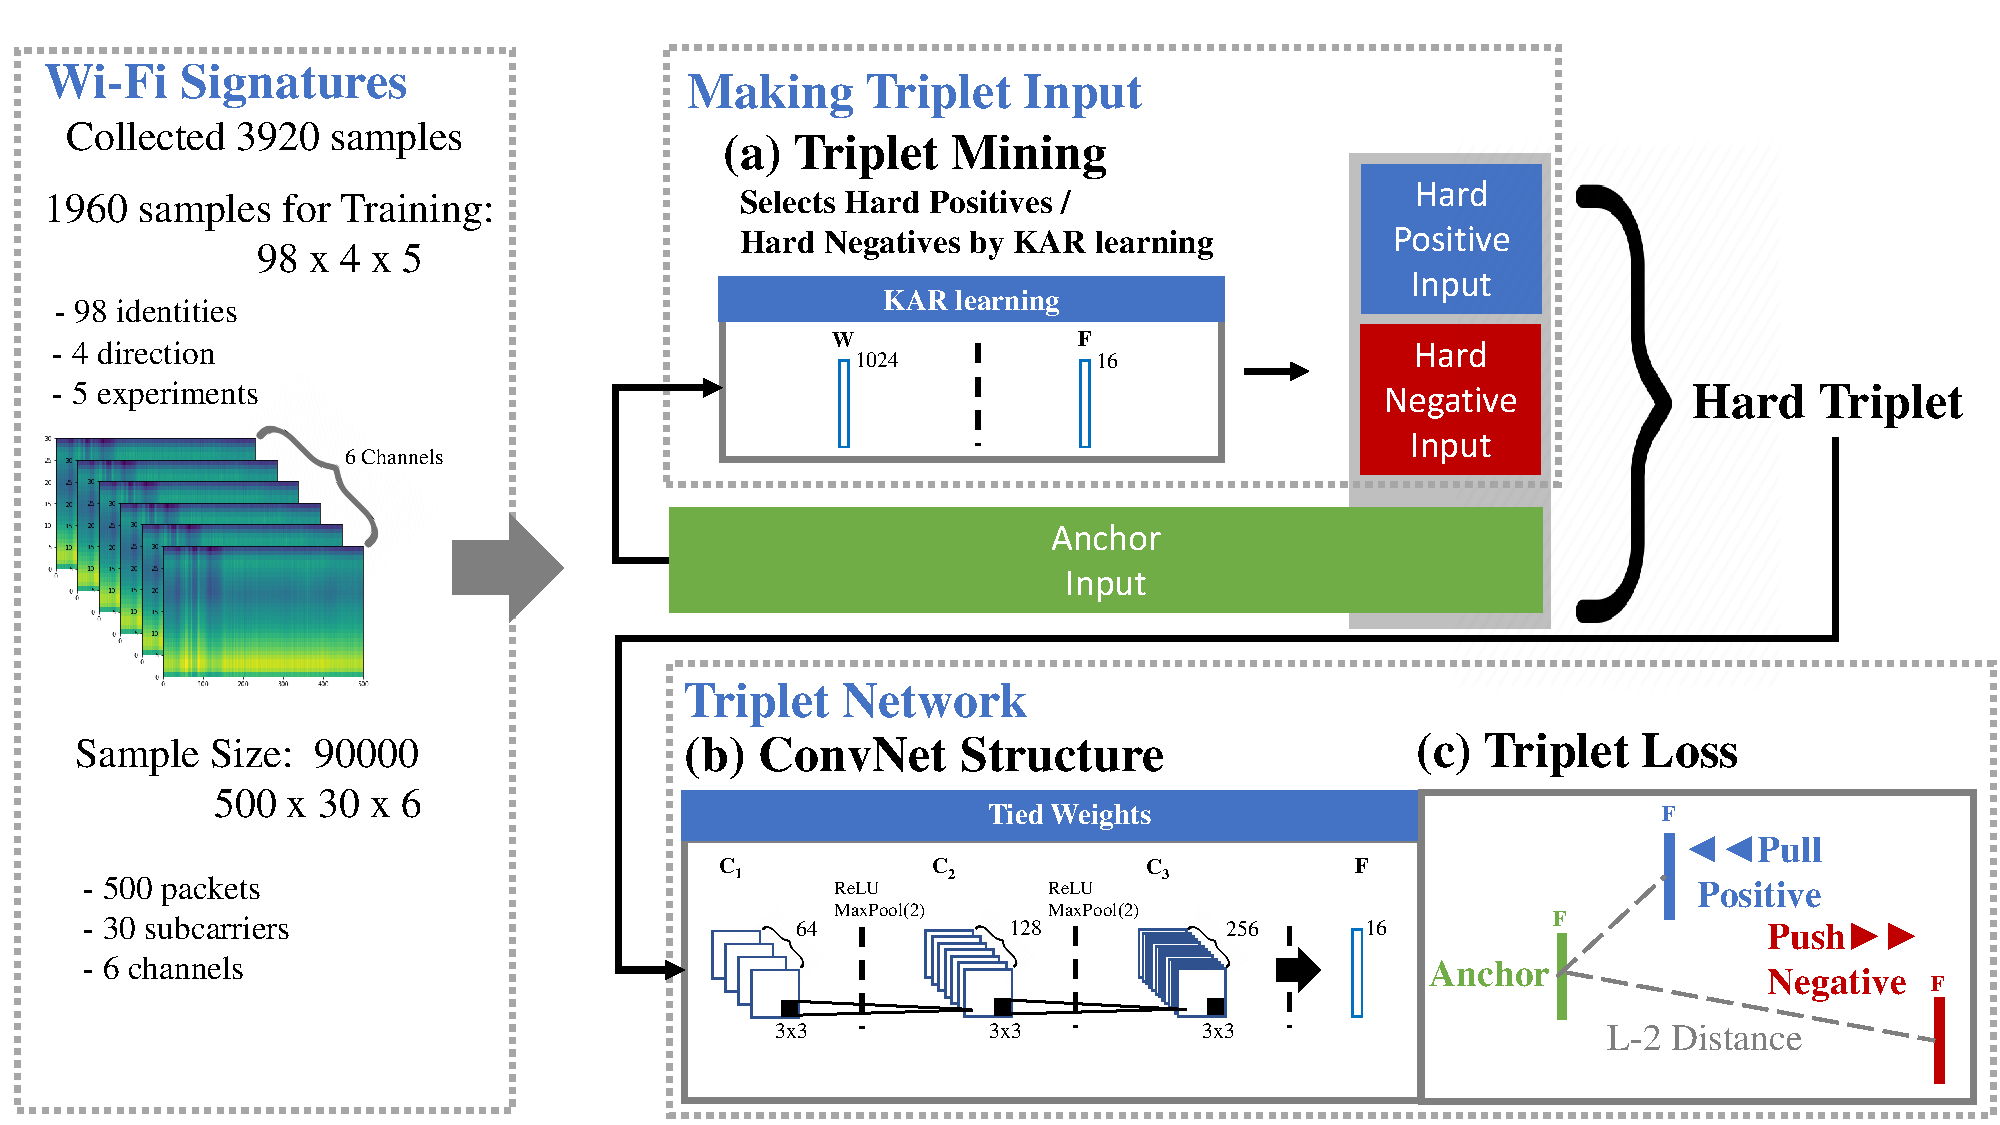
\includegraphics[width=\textwidth]
        {fig_system_overview_v1.pdf}
    \caption{An overview of the proposed methodology.} \label{fig1}
\end{figure*}
Figure~\ref{fig1} shows an overview of the proposed system. 
KAR space projection learning is used to mine hard samples from the training dataset to create triplets (Fig.~\ref{fig1}(a)). The anchor sample is randomly selected from the training dataset. The hard samples are those which are likely to be misclassified by the triplet network for a given anchor sample.
After the data is selected, the triplet network (Fig.~\ref{fig1}(b)) is trained based on the network output vector distance comparison (Fig.~\ref{fig1}(c)).
% following~
The following subsections discuss the triplet network architecture, triplet loss, and triplet mining using KAR space learning.

% 4.4.1. Triplet loss
\subsection{Triplet Loss}
% purpose
Triplet loss~\cite{hoffer2015deep} trains the ConvNet structure to learn the features that define data position in the feature space.
% Triplet input
Triplet inputs are composed of a combination of three samples, an anchor sample $x_0$, a positive sample $x_+$ and a negative sample $x_-$. The anchor sample, the reference for the triplet input, is selected from the training data set. The positive sample has the same identity as the anchor sample while the negative sample has a different identity.
% function
$dist\{f(x_0),f(x_+)\}$, the distance between the feature vectors of anchor $f(x_0)$ and positive sample $f(x_+)$ is larger than $dist\{f(x_0),f(x_-)\}$, the distance between feature vectors of the anchor and the negative sample plus a preset margin $\alpha$ to produce discriminative feature vectors. 
The distance measurement function is:
\begin{equation}
    dist\{f(x_0),f(x_-)\} - dist\{f(x_0),f(x_+)\} \geqq \alpha
    \label{triplet_condition}
\end{equation}
By using the $L2$ distance as the distance function, triplet loss is defined as:
\begin{equation}
    triplet\_loss = \sum_i^N max\left({ \left[ {\left\| {{f(x_0)} - {f(x_+)}} \right\|_2^2} - {\left\| {{f(x_0)} - {f(x_-)}} \right\|_2^2}  + \alpha \right]},0 \right),
    \label{triplet_loss}
\end{equation}
% need to make hard triplets
Note that if $dist\{f(x_0),f(x_-)\}$ is much larger than $dist\{f(x_0),f(x_+)\} + \alpha$, the output of the loss function is zero, significantly slowing deep network convergence. This condition is likely to occur if triplets are composed by randomly selecting training samples. Thus, triplet inputs must be selected that cause the loss function to produce a non-zero result.

% 4.4.2. Triplet mining
\subsection{Triplet Mining Based on KAR Space Learning}
% purpose
To train the triplet network faster, a sub-network for mining the hard positive and negative samples from the training dataset was trained.
% hard sample
The hard positive sample is likely to be misclassified as a negative sample by the triplet network (Fig.~ref{fig2}).
The distance between the feature vectors of the anchor and hard positive samples is larger than other positive samples.
The hard negative sample is likely to be misclassified as a positive sample because the distance between the feature vectors of the anchor and the hard negative sample is smaller than the difference between the feature vectors of the anchor and other negative samples.
Hard triplet inputs are made by combining hard positive and hard negative samples with selected anchor samples. Using hard triplets as triplet network inputs more easily, satisfies~\ref{triplet_condition}. However, before training the triplet network, it is impossible to identify hard samples.
% figure
\begin{figure*}[!ht]
    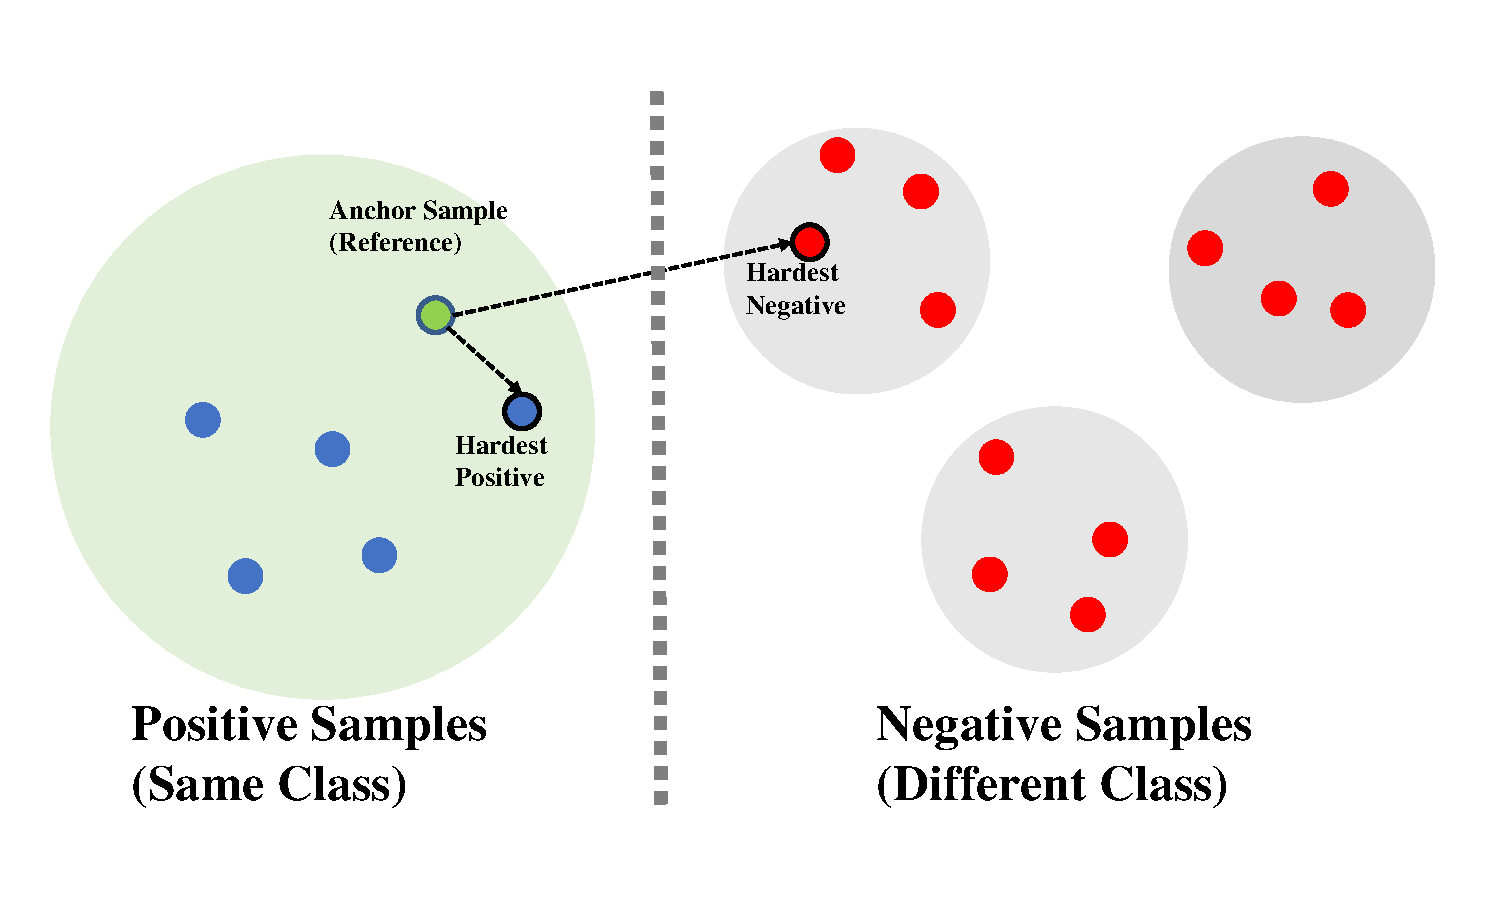
\includegraphics[width=\textwidth]
        {fig_hardsample_v1.pdf}
    \caption{Selection of hard samples.} \label{fig2}
\end{figure*}
% functions
In order to make hard triplets before tranining the triplet network, a smaller sub-network was trained before training the main triplet network.
This smaller sub-network was made of an MLP and was trained using KAR space learning. As KAR space learning has no backpropagation and no iterative learning process, it was trained all at once on the entire training dataset $X$. 
The sub-network output was defined as: 
\begin{equation}
    KAR\left(\mathbf{X}\right)=\sigma\left(\left[\mathbf{1},\sigma\left(\dots\left[\mathbf{1},\sigma\left(\left[\mathbf{1},\sigma\left(\mathbf{X}\cdot\mathbf{W}_{1}\right)\right]\mathbf{W}_{2}\right)\right]\dots\mathbf{W}_{(n-1)}\right)\right]\mathbf{W}_{n}\right).
\end{equation}
After training the sub-network, the hard samples were mined by measuring the $L2$ distance between every output vector of the sub-network and the output vector of anchor sample.
The sub-network output for a given anchor sample $x_0$ was $KAR(x_0)$. To mine hard-positive samples, one sample was selected from among the sub-network outputs for which the distance to the anchor feature vector $KAR(x_0)$ was larger than $t_+$. Hard-negative samples were chosen, from among the sub-network outputs for which the anchor feature vector was smaller than $t_-$.
The selected hard-positive and hard-negative samples satisfied the following properties, respectively:
\begin{equation}
    {\left\| {{KAR\left(\mathbf{x}_{0}\right)} - {KAR\left(\mathbf{x}_{+}\right)}} \right\|_2^2} \geq \mathrm{t}_{+}, 
    \label{thres_pos}
\end{equation}
\begin{equation}
    {\left\| {{KAR\left(\mathbf{x}_{0}\right)} - {KAR\left(\mathbf{x}_{-}\right)}} \right\|_2^2} \leq \mathrm{t}_{-},\label{thres_neg}
\end{equation}
If the hardest sample, outlier data is more likely to be selected than other data, resulting in an increased risk of overfitting~\cite{schroff2015facenet}.
To avoid this problem, the threshold for the hard-positive and the hard-negative samples were empirically chosen as the 25th and 75th percentiles of the distance between the anchor and sub-network outputs.

% 4.4.3. ConvNet Structures
\subsection{ConvNet Structures}
% Purpose
The three-dimensional format of the input signature signal is similar to that of image data, so deep ConvNet structures were used as the feature extractor. The ConvNets used in this thesis were made of three layers of ConvNets with triplet loss. Each layer of ConvNet shared their weights. 
% figure
\begin{figure*}[!ht]
    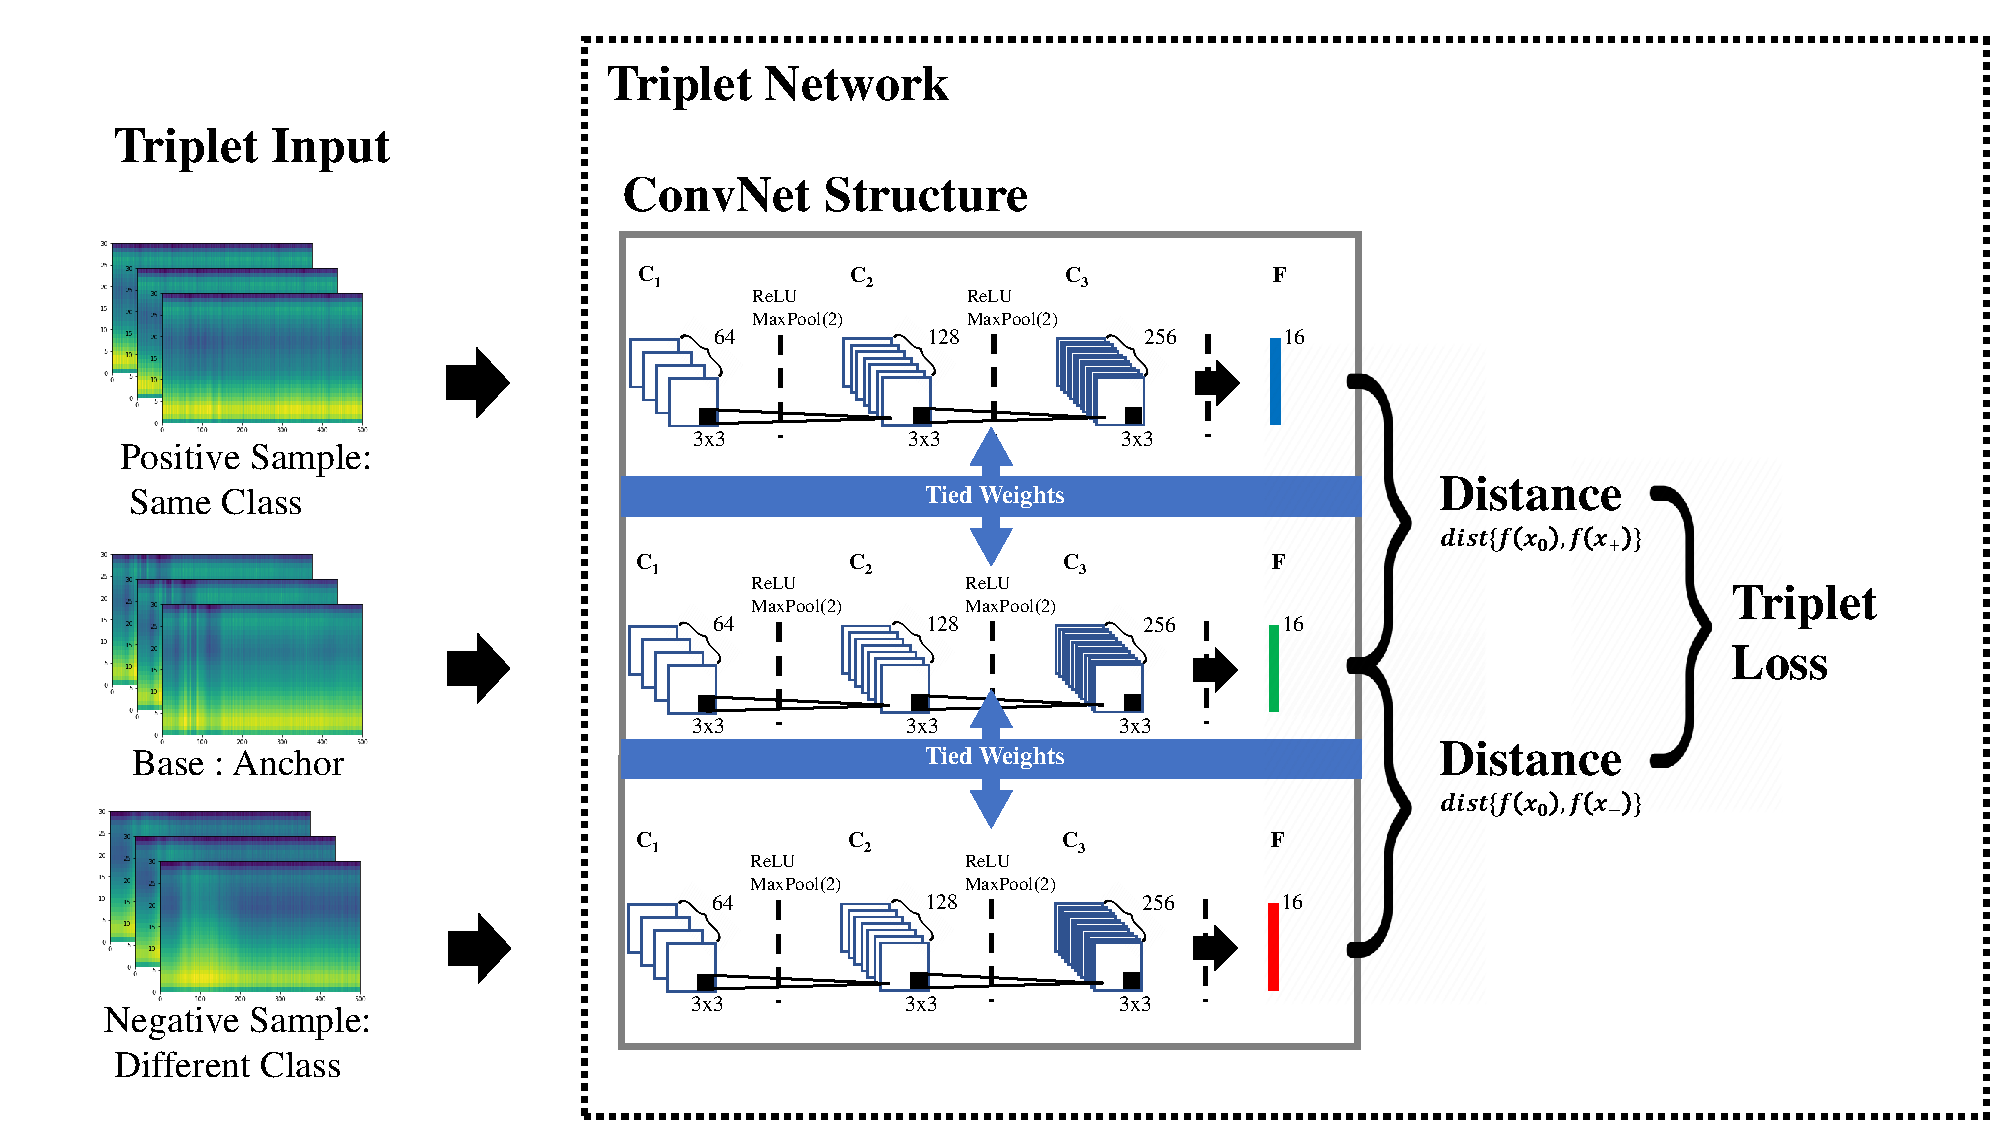
\includegraphics[width=\textwidth]
        {fig_convnet_v1.pdf}
    \caption{ConvNet structure.} \label{fig3}
\end{figure*}
% Structure
The ConvNets in this study consisted of three filters and a fully-connected output layer (Fig.~\ref{fig3}). The depth of the ConvNet filters was set at 64,128,256 with stride 1 and ReLU activation functions. The size of the fully-connected layer was 16. The fully-connected output layers were processed through sigmoid activation functions and were normalized according to the $L2$ distance.



\chapter{Experiments}\label{chapter:Experiments}
\label{chp:Experiments}
..
\section{Data set}
\label{sec:Dataset}
The Wi-Fi CSI signature dataset~\cite{moon2017air} at position 1 was implemented in our experiment to mesure the performance of our proposed system. These are in-house Wi-Fi signature datasets that comprise 980 signatures per direction, as shown in~\ref{tab_dataset}. The size of each sample was 500 x 30 x 6. 
We utilized only the magnitues of the complex values, since the signal have device firmware issues in their phase information~\cite{wang2015understanding}. 
\begin{table}
    \caption{Description of the Dataset.}
    \label{tab_dataset}
    \begin{tabular}{ccc}
    \hline
    Direction of signature & \# of identities & \# of data \\ 
    \hline
    1                      & 98               & 980        \\ 
    2                      & 98               & 980        \\ 
    3                      & 98               & 980        \\ 
    4                      & 98               & 980        \\ 
    \hline
    \end{tabular}
\end{table}

\section{Experimental Settings}
This section details the evaluation scenarios and experimental settings.

\subsection{Evaluation Scenarios}
%performance
In this paper, the verification performance of the proposed method was evaluated in three ways:
I) In the first experiment, verification performance was compared between the proposed system and other systems including handcraft and deep-learning based methods.
II) Under the second experiments, Comparison of convergence speed was conducted between the proposed system other deep-learning based methods. 
III) The third experiments was conducted to compare the performance degradation between the proposed system and other deep-learning based methods when using a small sized feature vectors. 
In order to compare the feature extraction performance of the proposed system with other deep-learning based methods, we visualized feature space into 2d euclidean space by using PCA. 
% handcraft
We compared the proposed system both with handcraft methods and deep learning based methods.
For handcraft methods, least square estimations (LSE)~\cite{duda2012pattern}, the principal components analysis(PCA)~\cite{turk1991eigenfaces} with LSE, the supprot vector machine~\cite{vapnik2013nature} and the total error minimization with the reduced multivariate polynomal~\cite{toh2003fingerprint,toh2008between} were used. We selected parameters that perform optimally in each handcraft methods. For LSE,SVM and TER, the input signatures were reduced to 500$\times$30 by averaging the subcarrier Axis. For PCA-LSE, input signature dimension was reduced to 40 following~\cite{moon2017air}. For SVM with Gaussian kernel function (RBF), the kernel's parameters $c$ and $\gamma$ were chosen by a grid search over the range $c\in\{0.01,1,10\}$ and $\gamma\in\{0.01/3000, 0.1/3000, 1/3000, 10/3000, 100/3000\}$. For TER, parameter M is chosen among $M\in\{1,2,3\}$ and set $\tau=\eta=0.5$ following~\cite{toh2008between}.
For comparison with deep learning based methods, Siamese network~\cite{koch2015siamese} and baseline triplet network~\cite{hoffer2015deep} were used.
%protocols
The verification performance was evaluated in terms of the Equal Error Rate (EER, \%). We implemented a random 5-runs of 2-fold cross validation tests.
Due to the hardware memory limitations, we used downsized negative pairs according to the number of positive data pairs for calculating the EER. The size of positive data pairs and downsized negative pairs were 18620.

%5.2.2. Parameter settings
\subsection{Parameter Settings}
% KAR structure
For the proposed system, the structure of the KAR learning MLP sub-networks is shown in~\ref{kar_structure}. We empirically chosen two layers size of 1024 and 16. The size of the second layer was equivalent as feature vectors of the proposed ConvNet. The weights in the layers weree initialized as a normal distribution of 0 to 1 before training.
We used $tan^{-1}$ as an active function following~\cite{toh2018analytic}.
\begin{table}[]
    \caption{The network structure of KAR space learning.}
    \label{kar_structure}
    \centering
    \begin{tabular}{|l|l|l|}
    \hline
    Layer   & Size     & Activation \\ \hline
    Input   & 500$\times$30$\times$6 &            \\
    Fully-Connected 1 & 1$\times$1$\times$1024 & $\sigma = {tan}^{-1}$     \\
    Fully-Connected 2 & 1$\times$1$\times$16  & $\sigma = {tan}^{-1}$     \\
    Output  & 1$\times$1$\times$50   &            \\ \hline
    \end{tabular}
\end{table}
% conv structure
We used the same ConvNet structure shown in~\ref{conv_structure} and parameter settings for the proposed system and the deep-learning based methods. The CovNet structure consists of 3  convolution filters size of 3$\times$3 and stride 1. A ReLU activation function and 2$\times$2 max-pooling layers is applied between the filters. The depth of each layer was chosen as \{64,128,256\}. The output layer with sigmoid activation was regularized using $L2$ penalty of 0.0001. The size of the final feature vectors was 16.
\begin{table}[]
    \caption{The structure of ConvNet model.}
    \label{conv_structure}
    \centering
    \begin{tabular}{|c|c|c|c|}
    \hline
    Layer     & Activation & Kernel / Stride & Input Size \\ \hline
    Conv 1    & ReLU       & (3$\times$3)$\times$64/1      & 500$\times$30$\times$6   \\
    MaxPool 1 &            & (2$\times$2)/1         & 500$\times$30$\times$64  \\
    Conv 2    & ReLU       & (3$\times$3)$\times$128/1     & 250$\times$15$\times$64 \\
    MaxPool 2 &            & (2$\times$2)/1         & 250$\times$15$\times$128 \\
    Conv 3    & ReLU       & (3$\times$3)$\times$256/1     & 125$\times$8$\times$128  \\
    MaxPool 3 &            & (2$\times$2)/1         & 125$\times$8$\times$256  \\
    Fully-Connected     & Sigmoid    & 16             & 63$\times$4$\times$256   \\
    L-2 Norm  &            &                 & 1$\times$1$\times$16    \\
    Concat    &            &                 & 1$\times$1$\times$16    \\ \hline
    \end{tabular}
\end{table}
% traning parameters
The parameter settings for traning the deep learing network was 
learning rate of 0.0005, the number of iteration as 3000, and set the mini-batch size as 32. We used adam optimatizer for calculating the loss function. We initialized the ConvNet structures following ~\cite{koch2015siamese} before training. For convolution filters, we used a normal distribution of 0 mean and standard deviation of 0.0001. For the biases, parameters for normal distribution was 0.5 mean and standard deviation of 0.01. For calculating triplet loss, we set the alpha value as 0.5.

%5.3. Experimental results
\section{Experimental Results}
%5.3.1. verification performance
\subsection{Performance}
For experiment I,~\ref{tab_performance} shows the average EER from 5-runs of 2-fold cross-validation tests under the optimal parameter settings. As shown in Table~\ref{tab_performance}, the proposed system shows best performance among the handcraft and deep-learning based methods with 19.35\% EER.
Deep learning based methods performed better performance than handcraft methods since they were able to utilize the entire input signal, and their ability to feature extraction were better than handcraft methods.
\begin{table}[!h]
    \caption{Performance benchmarking with respect to the best EER (\%) averaged from five runs of two-fold cross-validation test on Wi-Fi CSI signature dataset.}\label{tab_performance}
    \centering
    \begin{tabular}{|c|c|c|}
    \hline
    Methology   &   Best EER (\%) &   Condition   \\  \hline
    LSE &   48.44   &  - \\ 
    PCA-LSE    &   30.79   &  Reduced dimension=40    \\
    SVM (Linear) &   28.23   &   c=1 \\
    SVM (RBF)    &   24.31   &   c=1, $\gamma$=0.01/3000 \\
    TER-RM2 &   35.84   &  M=1,$\tau$=$\eta$=0.5   \\     \hline
    Siamese network  &   23.53   &   lr=0.00005  \\
    Baseline triplet network &   20.34   &   lr=0.00005, $\alpha$=0.1  \\
    \textbf{Proposed system} &   \textbf{19.35}   &  \textbf{lr=0.00005, $\alpha$=0.1}  \\
     \hline
    \end{tabular}
\end{table}

%roc
As shown in~\ref{fig_roc}, the proposed system also showed the widest Area under ROC curve (AUC).
\begin{figure*}[!ht]
    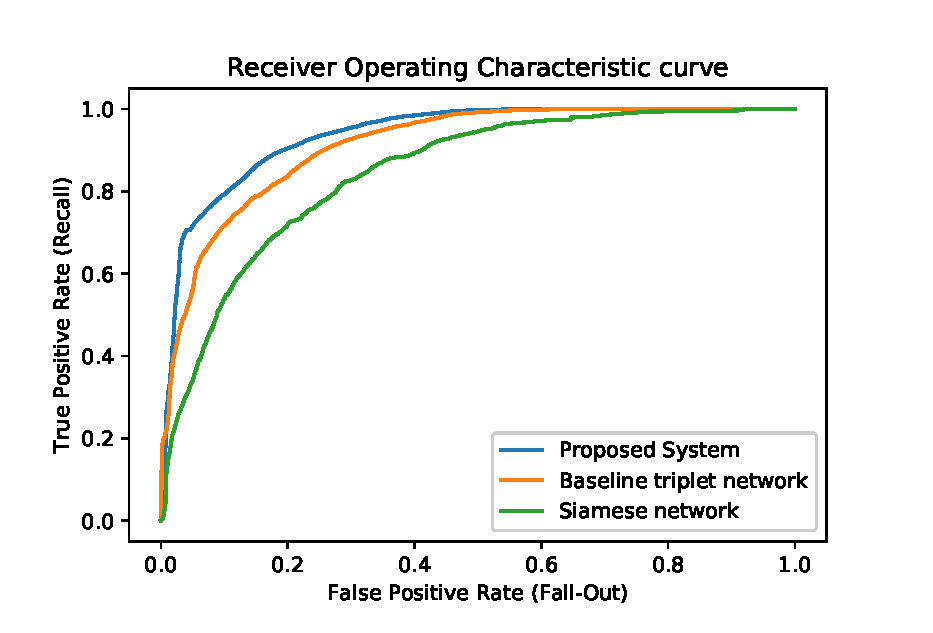
\includegraphics[width=\textwidth]{fig_roc_v15.eps}
    \caption{Normalized training loss curve.} \label{fig_roc}
\end{figure*}
 %5.3.1. conv speed
~\ref{fig_loss} shows the convergence of the normalized loss function during the training. The convergence speed of the proposed system was the fastest among the deep learning-based methods, meaning that KAR running has accelerated the learning speed.
\subsection{Convergence speed}
 \begin{figure*}[!ht]
    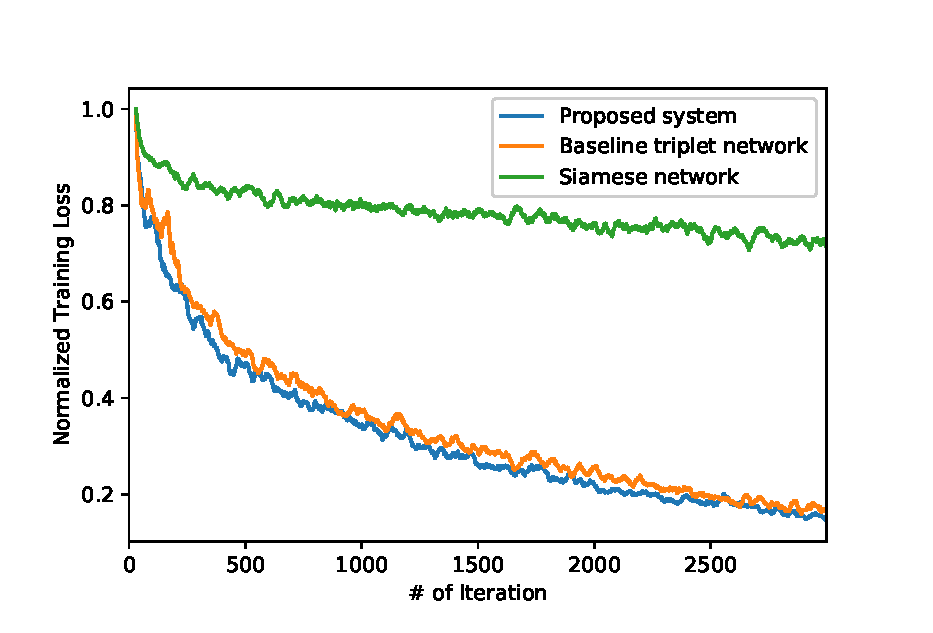
\includegraphics[width=\textwidth]{normalized_loss_curve_ma30_v3.eps}
    \caption{normalized training loss trends} \label{fig_loss}
\end{figure*}
%5.3.2. feature vector
\subsection{Effect of the size of Feature Vector}
- Case3) FC layer
○ Picture
○ The smaller the mapping to a characteristic space, the lower the performance degradation of the proposed method is.
§ Reason 1: Triplet network has better space placement capability than Siamese
Reason 2: Triplet network with KAR learning is better performance

\begin{table}[]
    \centering
    \begin{tabular}{|l|l|l|l|l|}
    \hline
    Size of the Feature Vector & 16    & 8     & 4     & 2     \\ \hline
    Siamese network            & 20.34 & 22.05 & 29.39 & 34.26 \\ \hline
    Baseline triplet network   & 18.37 & 19.52 & 19.20 & 24.76 \\ \hline
    Proposed system            & 16.92 & 18.03 & 18.08 & 26.64 \\ \hline
    \end{tabular}
\end{table}
\begin{figure}[!ht]
    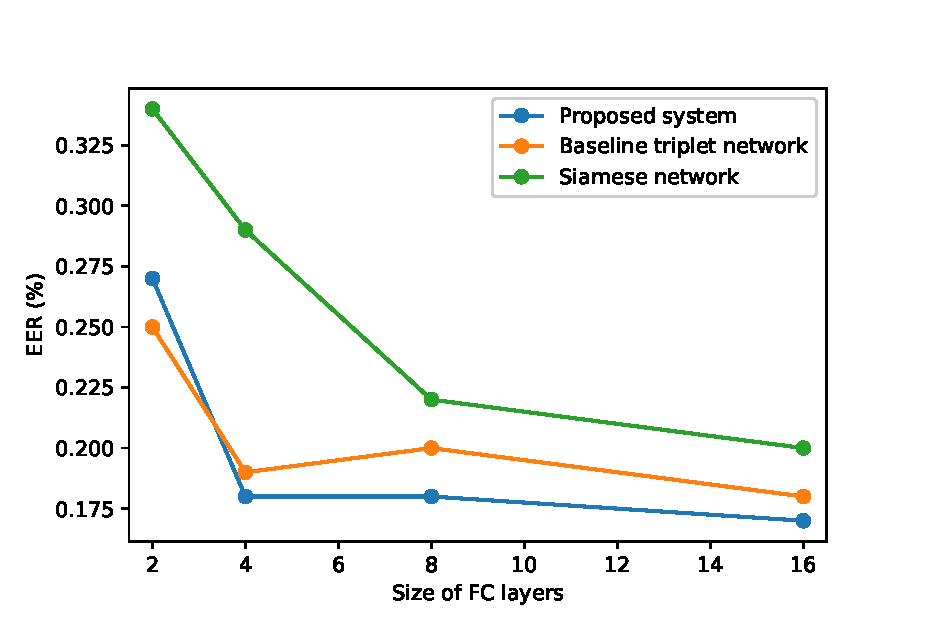
\includegraphics[width=\textwidth]{fclayer_v1.eps}
    \caption{Size of FC layer.} \label{fclayer}
\end{figure}

\begin{figure}[!ht]
    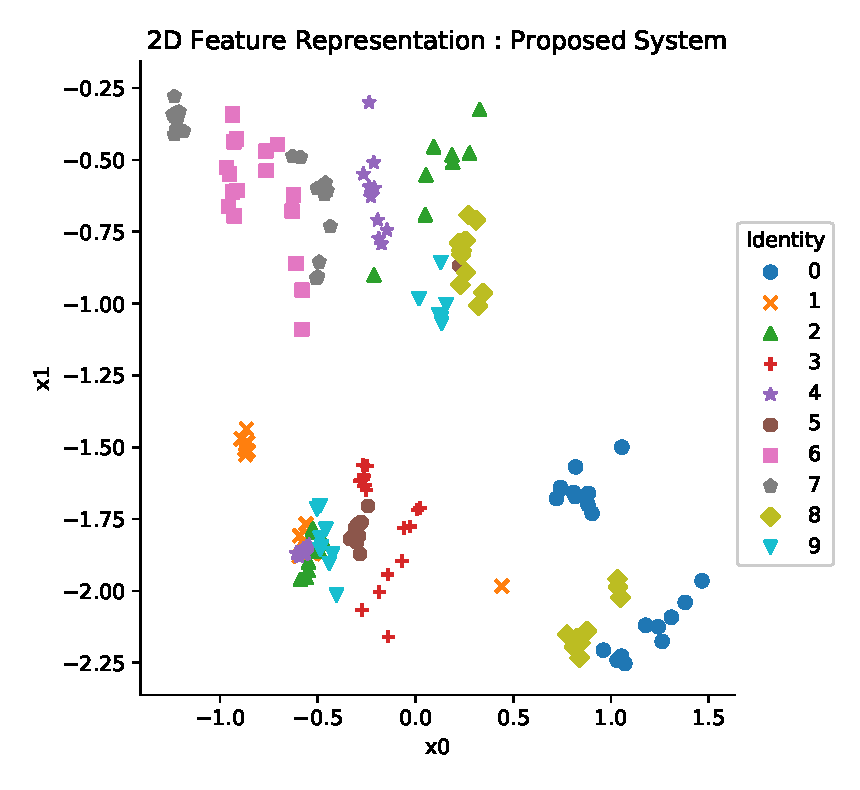
\includegraphics[width=\textwidth]{fig_2d_triKAR_10_v1.eps}
    \caption{2D Feature Representation : Proposed System.} \label{fig_2d_triKAR_10}
\end{figure}
\begin{figure}[!ht]
    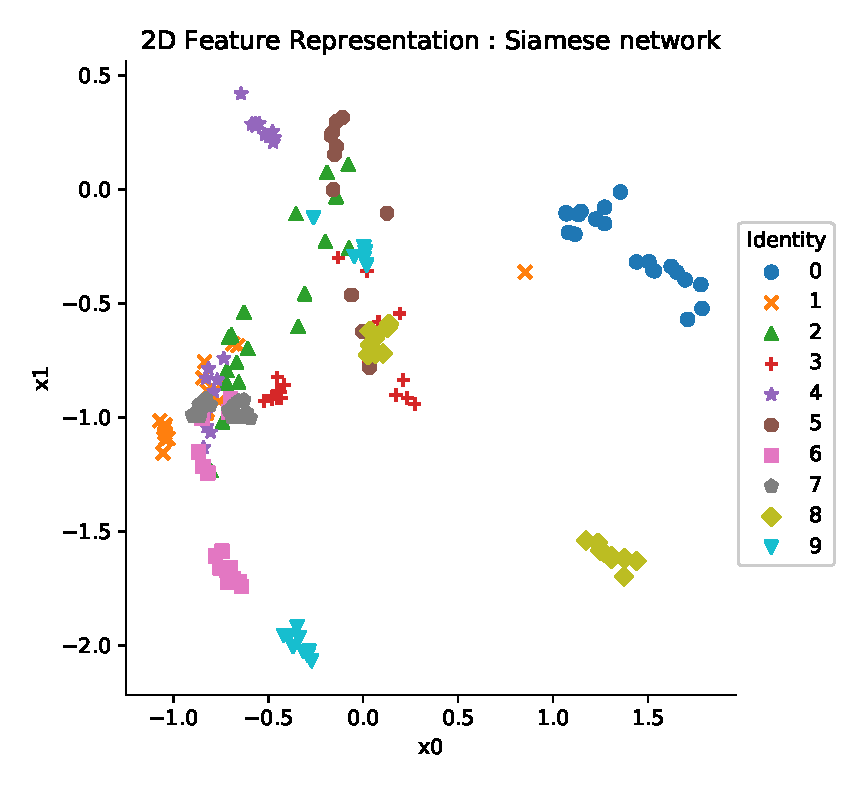
\includegraphics[width=\textwidth]{fig_2d_tribase_10_v1.eps}
    \caption{2D Feature Representation : Baseline triplet network.} \label{fig_2d_tribase_10}
\end{figure}
\begin{figure}[!ht]
    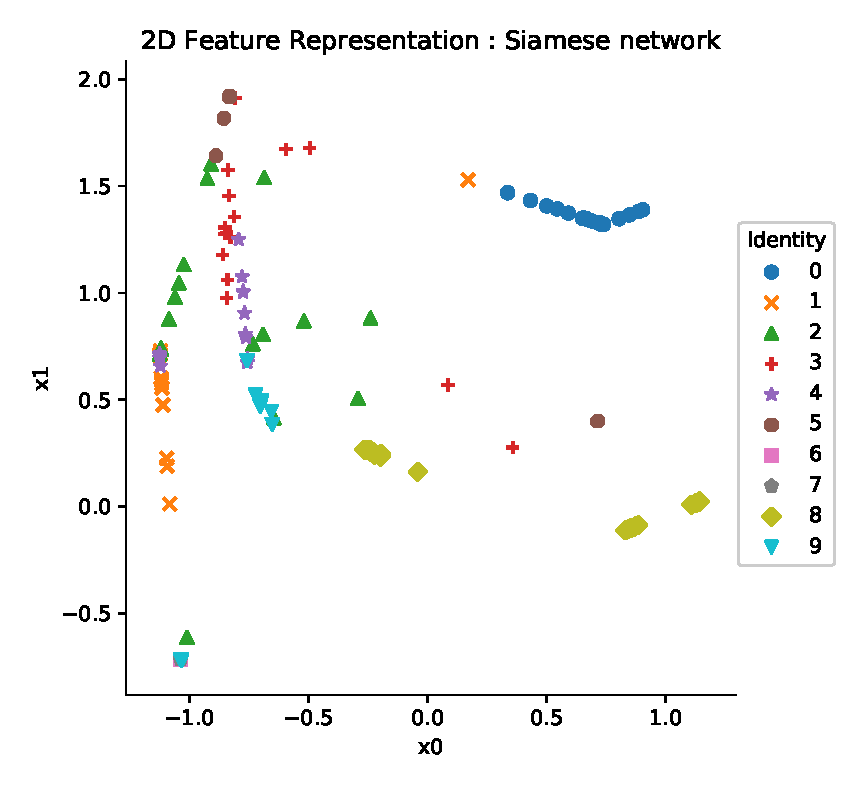
\includegraphics[width=\textwidth]{fig_2d_siam_10_v1.eps}
    \caption{2D Feature Representation : Siamese network.} \label{fig_2d_siam_10}
\end{figure}

\chapter{Conclusion}\label{chapter:Conclusion}
\label{chp:Conclusions}
\section{Conclusions}
...

\section{Future Works}
...
\begin{enumerate}
	\setlength{\itemsep}{1pt}
	\item Recognizing the in-air signature written along non-LOS. 
	\item Repeating the same data acquisition experiments in a different place
	\item Studying identification performances when multiple people are staying in the same room.
	\item To secure a reliable identification system, spoofing attack scenario should be investigated. 
\end{enumerate} 

%\begin{appendix}
%\input{appendix}
%\end{appendix}

%\bibliography{main}
%\addcontentsline{toc}{chapter}{\protect\numberline{}
%    \hspace*{-0.29in} Bibliography}
%\input{bibliography}

\addcontentsline{toc}{chapter}{\protect\numberline{}
    \hspace*{-0.29in} Bibliography}
%\bibliographystyle{IEEEtran}
\bibliographystyle{unsrt}
\bibliography{bib_thesis_HERO}

\clearpage
\addcontentsline{toc}{chapter}{\protect\numberline{}
    \hspace*{-0.29in} Summary (in Korean)}
{\large
	\noindent 국문요약}\\[11pt]
\begin{center}
	\vskip 2em \Large 와이파이 신호를 이용한 공중 서명 인식 시스템 
\end{center}
\vskip 2em
...

\vspace{\stretch{1}}

\noindent
\hrulefill\\
핵심되는 말:
\parbox[t]{0.8\textwidth}
{...}


%\newpage % Response Note %%%%%%%%%%%%%%%%%%%%%%%%%%%%%%
%\input{response}

\end{document}
